\documentclass[11pt]{article}
\usepackage{amsmath,textcomp,amssymb,geometry,graphicx,enumerate}
\usepackage{tabu}
\usepackage{algorithm} % Boxes/formatting around algorithms
\usepackage[noend]{algpseudocode} % Algorithms
\usepackage{graphicx}
\usepackage{caption}
\usepackage{subcaption}
\usepackage{siunitx}

\def\Name{Sam Holladay}  % Your name
\def\SID{24194437}  % Your student ID number
\def\Homework{8} % Number of Homework
\def\Session{Fall 2015}


\title{EE230C Final Project: Monolayer Graphene Field-Effect Transistor}
\author{Sam Holladay, Saavan Patel, and Charles Zhang}
\markboth{EE230C: Holladay, Patel, and Zhang}{EE230C: Holladay, Patel, and Zhang}
\pagestyle{myheadings}
\date{}

\newenvironment{qparts}{\begin{enumerate}[{(}a{)}]}{\end{enumerate}}
\def\endproofmark{$\Box$}
\newenvironment{proof}{\par{\bf Proof}:}{\endproofmark\smallskip}

\textheight=9in
\textwidth=6.5in
\topmargin=-.75in
\oddsidemargin=0.25in
\evensidemargin=0.25in


\begin{document}
\maketitle

\section*{i.} The experimental performance of several sub-100 nm graphene transistors were demonstrated by Wu for RF purposes\cite{wu2010}. The topology of these graphene devices is shown in Figure 1. The current-voltage characteristics of the 70 nm FETs were measured at both room temperature and low temperature. The performance of the FETs were also modeled, and Figure 2a and 2b shows a comparison of the experimental and modeled current $I_d$ vs the gate voltage $V_g$ and the drain voltage $V_d$, respectively. 
\begin{figure}[h!]
\centering 
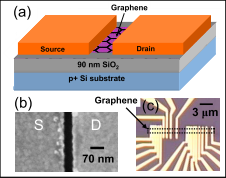
\includegraphics[width=0.3\textwidth]{paper1_fet.png}
\caption{(a) Schematic view of Wu's back-gated graphene FET, (b) SEM image of metal contacts of a 70nm device and (c) optical image of the fabricated devices.}\label{fig:FET}
\end{figure}

Experimental data of the contact resistance was also collected at different temperatures, as seen in Figure 3. Mobility data vs temperature was also collected, shown in Figure 4.

\begin{figure}[h!]
\centering 
\begin{subfigure}[b]{0.3\textwidth}
        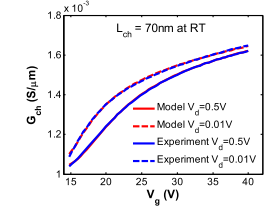
\includegraphics[width=\textwidth]{paper1_idvg3.png}
        \caption{Comparison of experiment and model of the transfer characteristics.}
        \label{fig:Idvg}
\end{subfigure}
\begin{subfigure}[b]{0.3\textwidth}
        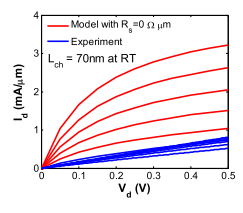
\includegraphics[width=\textwidth]{paper1_idvd3.png}
        \caption{Modeled output characteristics with $R_s=0$ vs experiment.}
        \label{fig:Idvd}
\end{subfigure}
\caption{Measurements by Wu of 70 nm device at room temperature}\label{fig:animals}
\end{figure}

\begin{figure}[h!]
\centering 
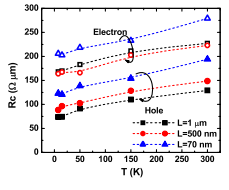
\includegraphics[width=0.3\textwidth]{paper1_contactres.png}
\caption{Contact resistance $R_c$ vs T from devices with different channel length, from 1 $\mu$m to 70 nm.}\label{fig:FET}
\end{figure}

\begin{figure}[h!]
\centering 
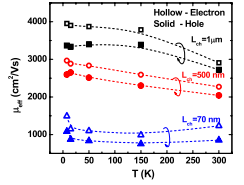
\includegraphics[width=0.3\textwidth]{paper1_mobilitydata.png}
\caption{Effective electron and hole mobility $\mu_{eff}$ vs T from devices with different channel length, from 1 $\mu$m to 70 nm.}\label{fig:FET}
\end{figure}

Additionally, in 2011 Meric et al \cite{meric2011} took a comprehensive look at channel-length scaling of graphene FETs, including several with channel lengths under 100 nm. Their graphene FET design is similar to Wu's, and is shown in Figure 5.

\begin{figure}[h!]
\centering 
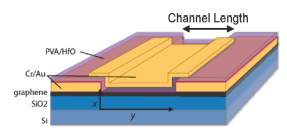
\includegraphics[width=0.3\textwidth]{meric_fet_layout.png}
\caption{Schematic view of Meric's graphene FET.}\label{fig:FET}
\end{figure}

\section*{ii.} To calculate the current-voltage characteristics, the bandstructure of graphene must be derived. The Hamiltonian matrix is first constructed, and the eigenvalues are determined computationally. Using the method of Linear Combination of Atomic Orbitals as described in Slater and Koster \cite{slaterkoster1954}, we construct the on and off diagonal terms Hamiltonians. A six-band tight-binding model is used, which includes the $p_z,d_{yz}, d_{zx}$ orbitals. These have binding energies described by Boykin \cite{boykin2011}. The band structure is generated by finding the eigenvalues of the 6x6 Hamiltonian generated by the equation:

$H = H_{on} + H_{off}e^{i\vec{k}\vec{t_1}} + H^T_{off}e^{-i\vec{k}\vec{t_1}} + H_{off}e^{i\vec{k}\vec{t_2}} + H^T_{off}e^{-i\vec{k}\vec{t_2}}$

Here, the vectors $\vec{t_1}$ and $\vec{t_2}$ represent the basis vectors for the graphene unit cell, as denoted in Figure 5a. The $\vec{k}$ is the momentum vector, which we allow to take values over the entire first Brillouin zone, displayed in Figure 6b. 

\begin{figure}[h!]
\centering
\begin{subfigure}[b]{0.3\textwidth}
        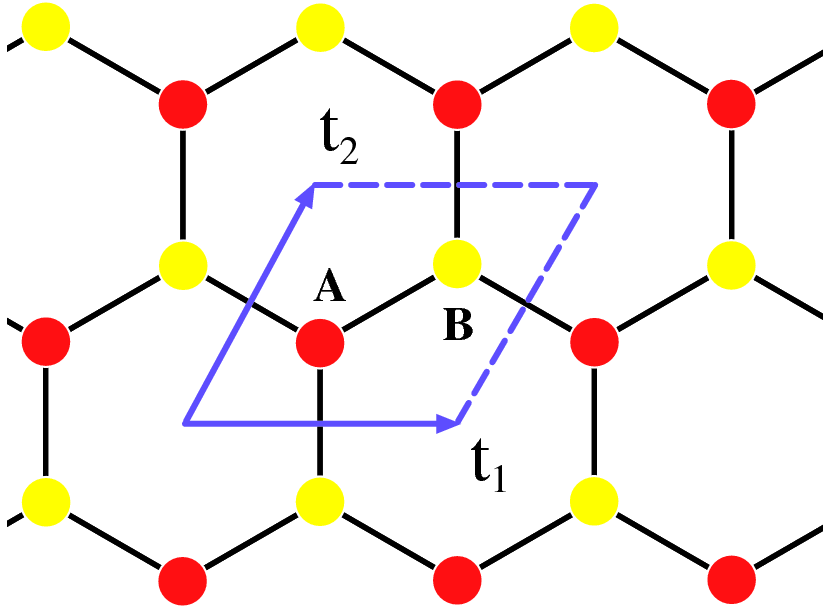
\includegraphics[width=\textwidth]{graphene_unit_cell.png}
        \caption{The graphene unit cell, with translation vectors. Different colors represent different atoms in the unit cell.}
\end{subfigure}
\begin{subfigure}[b]{0.3\textwidth}
        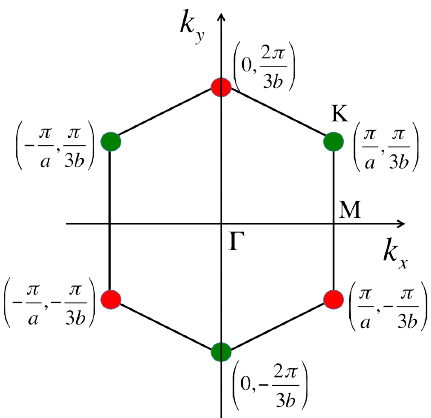
\includegraphics[width=\textwidth]{Figure-5-Graphene-first-Brillouin-zone}
        \caption{Brillouin zone of graphene, showing the $\Gamma$, K, and M points.}
        \label{fig:Idvd}
\end{subfigure}
\caption{Physical structure of graphene}\label{fig:animals}
\end{figure}

The calculated bandstructure is presented in Figure 7a, with the bandstructure from Boykin presented side-by-side for comparison

\begin{figure}[h!]
\centering
\begin{subfigure}[b]{0.3\textwidth}
    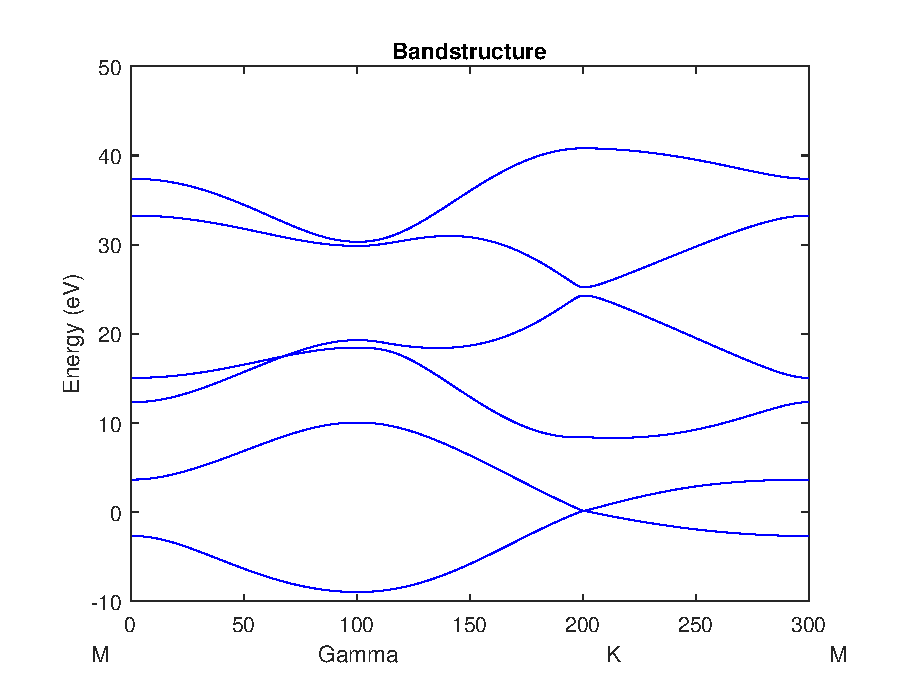
\includegraphics[width=\textwidth]{Bandstructure.eps}
\caption{Calculated bandstructure using 6-band tight binding model}
\end{subfigure}
\begin{subfigure}[b]{0.3\textwidth}
    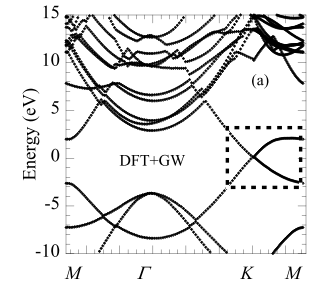
\includegraphics[width=\textwidth]{paper1_bandstructure.png}
\caption{Bandstructure from Boykin}
\end{subfigure}
\end{figure}

Around the Dirac point our calculated bandstructure closely matches the bandstructure from literature as seen in Figure 8, showing graphene's characteristic linear dispersion relation at low voltages:

\begin{figure}[h!]
\centering
\begin{subfigure}[b]{0.3\textwidth}
    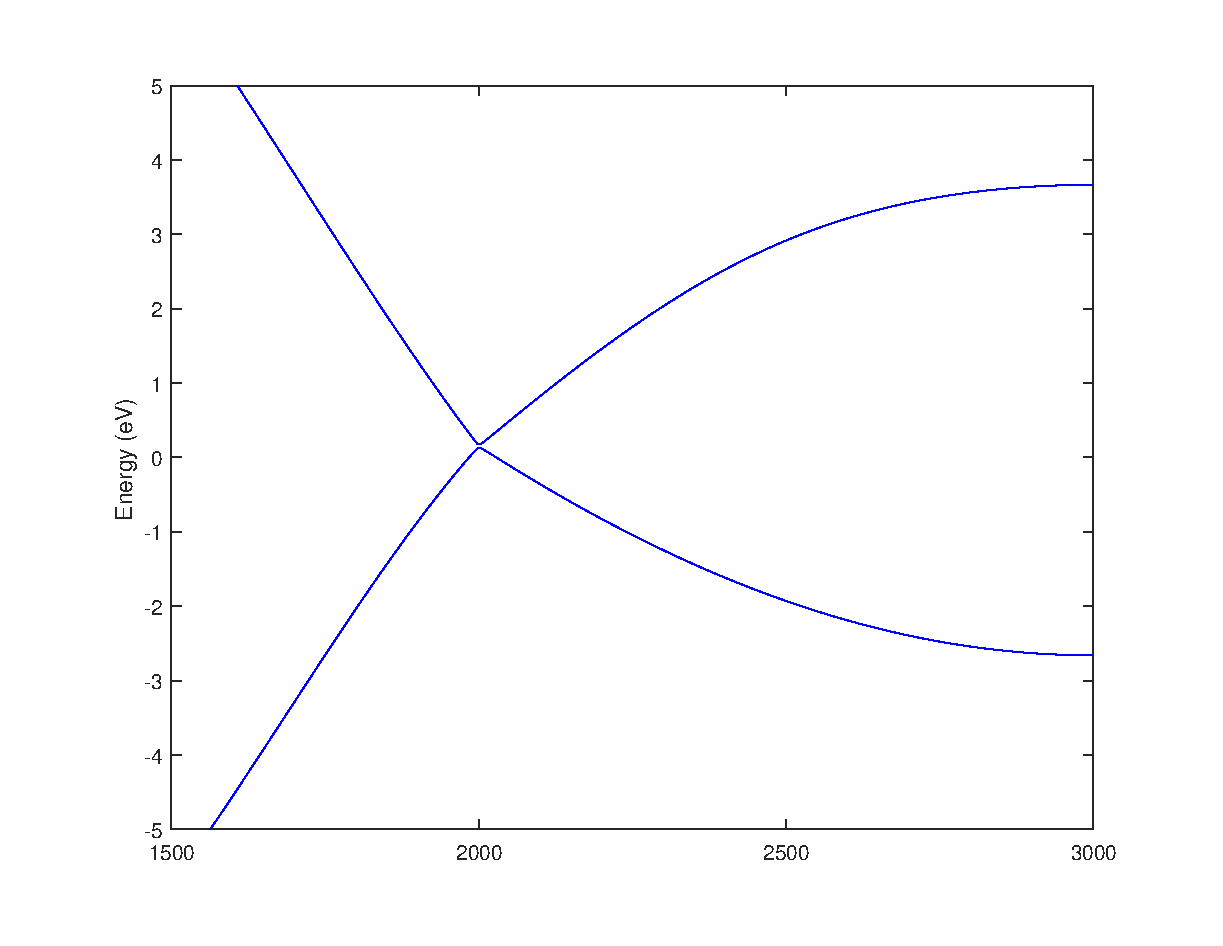
\includegraphics[width=\textwidth]{DiracPoint.eps}
\caption{Calculated bandstructure}
\end{subfigure}
\begin{subfigure}[b]{0.3\textwidth}
    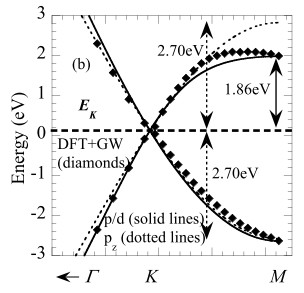
\includegraphics[width=\textwidth]{paper_diracpoint.png}
\caption{Bandstructure from Boykin}
\end{subfigure}
\caption{Comparison of calculated and literature bandstructures around Dirac point}
\end{figure}

For the dimensions of the modeled transistor, we assumed a width of $W=1\mu$m, and during parts ii-iv assumed a channel length of $L=70 nm$ to compare the simulation results to experimental results from Wu. 

To derive the current-voltage characteristics of the transistor, we proceed from the fundamental quasi-ballistic equation for current:

$$I_d = -ew(\sum_{k_x>0, ky}f_{k}v_{k} - \sum_{k_x<0, ky}f_{k}v_{k})$$

This includes back-scattering of electrons going back over the barrier from the drain. We recall the expressions for $f_{k}$ and $v_{k}$:

$$f_{k}=\frac{1}{1+exp(\frac{\mathcal{E}_{k}(k_x,k_y) - \mu}{k_BT})}, \hspace{1em} v_{k} = \frac{1}{\hbar}\nabla_k(E)= \frac{1}{\hbar}(\frac{dE}{dk_x}+\frac{dE}{dk_y})$$

Here, since we are working from the numerical values of the rigorous bandstructure, $v_k$ is calculated numerically from the gradient of $E_k$ with respect to both $k_x$ and $k_y$. Analytic approximations for band structure are shown below, in section iii.

After deriving the bandstructure, the current can be determined computationally after converting the sum into a double integral by taking the limit of $k_x$ and $k_y$ to 0 and normalizing by $\frac{1}{4\pi^2}$:

$$\sum_{k_x>0, ky}f_{k}v_{k} =\int_{0}^{\infty}dk_xdk_yv_{k}f_{k} = \int_{0}^{\infty}\frac{1}{4\pi^2}dk_xdk_y\frac{1}{1+exp(\frac{\mathcal{E}_{k} - \mu_S}{k_BT})}\frac{1}{\hbar}\nabla_k(E)$$

With the corresponding expression for current from electrons going back over the barrier from the drain to the source:

$$\sum_{k_x<0, ky}f_{k}v_{k} =\int_{-\infty}^{0}dk_xdk_yv_{k}f_{k} = \int_{-\infty}^{0}\frac{1}{4\pi^2}dk_xdk_y\frac{1}{1+exp(\frac{\mathcal{E}_{k} - \mu_D}{k_BT})}\frac{1}{\hbar}\nabla_k(E)$$

To simplify calculations, $\mu_S$ is set to 0 as the reference point for the potential. This takes care of current from electrons. To derive the total current in graphene, however, the hole current must also be taken into account, using the similar formula

$$I_{D-holes} = 2ew(\sum_{k_x<0, ky}f_{k}v_{k} - \sum_{k_x>0, ky}f_{k}v_{k})$$

because holes flow the opposite direction of electrons. While the velocity $v_k$ is calculated the same for holes due to graphene's symmetric dispersion relation, the Fermi function $f_k$ changes in the usual fashion:

$$f_{kholes}=1-f_{kelectrons}$$

Then, proceeding the same way, the hole current is calculated and the total current $I_d$ is

$$I_d = I_{delectrons}+I_{dholes}$$

Thus a quasi-ballistic current dependent on the drain voltage $I_d$ is determined, with contact resistance not yet taken into account. This current is shown in Figure 9.

\begin{figure}[h!]
\centering 
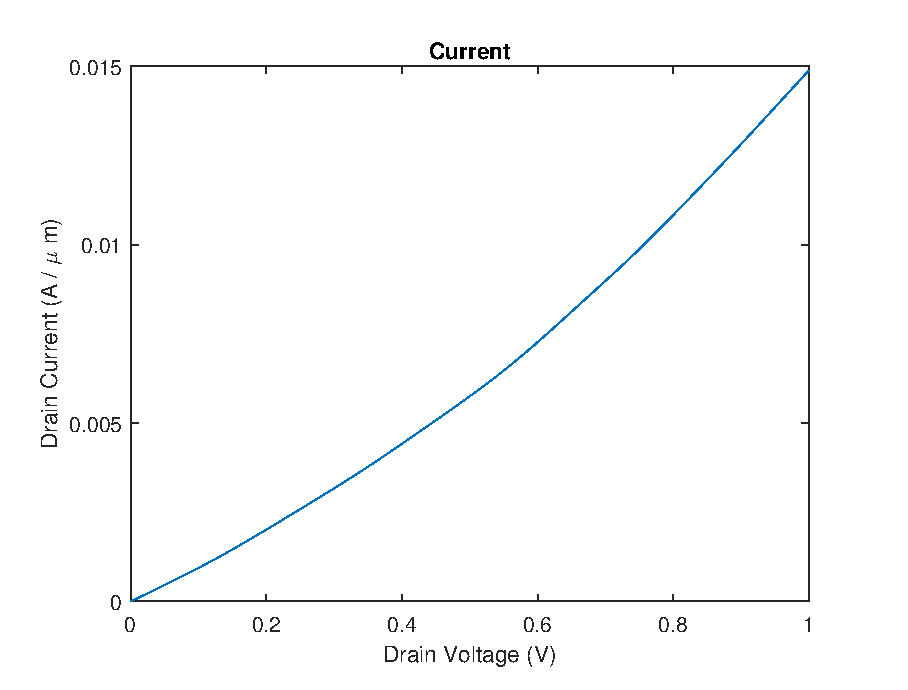
\includegraphics[width=0.4\textwidth]{current.eps}
\caption{Drain current $I_d$ vs drain voltage $V_d$, without any contact resistance.}\label{fig:FET}
\end{figure}

In contrast with the model results from Wu, $I_d$ does not saturate around 1 V. However, this is a well-documented effect in graphene; Chauhan noted a nearly linear $I_d-V_d$ relationship with a "characteristic kink" in the curve around $V_d=0.5$\cite{chauhan2011}. Meric explains this kink as a result of an ambipolar channel in graphene transistors \cite{meric2011}; this ambipolarity is supported in the $I_d-V_g$ plots displayed later in this report, where the $I_d-V_g$ characteristics are symmetric around 0. For low applied $V_ds$, holes carry most of the current across the length of the channel; starting at around $V_{kink}$, the vanishing carrier density produces a "pinch-off region" in the drain that produces the kink. For voltages greater than the kink, an electron channel forms at the drain, and current flows normally. The kink is small and hard to see in our results, but is still present.

\begin{figure}[h!]
\centering
\begin{subfigure}[b]{0.3\textwidth}
    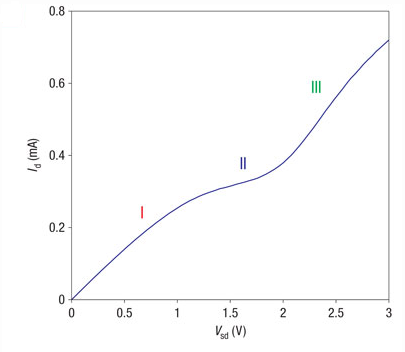
\includegraphics[width=\textwidth]{meric_kink_plot.png}
\caption{Region I: Mainly hole current, Region II: "Kink," Region III: Electron and hole current flow}
\end{subfigure}
\begin{subfigure}[b]{0.3\textwidth}
    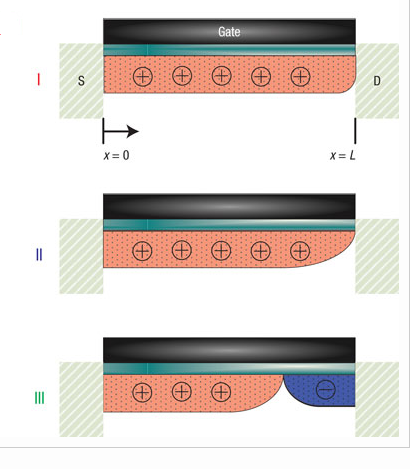
\includegraphics[width=\textwidth]{meric_kink_explanation.png}
\caption{Kink effect on $I_d-V_d$ plot correspond to different regions of carrier concentration in the channel}
\end{subfigure}
\caption{Description by Meric of linear $I_d-V_d$ characteristics and "kink" seen in graphene FETs}
\end{figure}

This take care of the current's variation with just the drain voltage $V_d$. To implement gate control by the gate voltage $V_g$, the potential at the top of the barrier between source and drain is self-consistently with the number of carriers at the top of the barrier. For this model, charges in the channel are provided through thermionic emission from the source and drain contacts. Both electron and hole charges are taken into account to explain both positive and negative bias behavior. 

At equilibrium the concentration of carriers is the following:
$$N0 = \int_{-\infty}^{\infty}{D(E)f(E-Ef)dE}$$
where $D(E)$ is the density of states calculated from the band structure, and $f(E)$ is the fermi function at that energy level. This is used as an initial guess for the self consistent solution. We use the following equations, as described by Rahman \cite{ballistic2002}:

\begin{enumerate}
\item $U_{TOB} = q\phi(\frac{C_G}{C_T} + \frac{C_D}{C_T}) + q^2\frac{N-N_0}{C_t}$ 
\item $N = \int_{-\infty}^{\infty}{D(E)f(E+U_{TOB}-\mu_s)} + \int_{-\infty}^{\infty}{D(E)f(E+U_{TOB}-\mu_d)}$
\end{enumerate}

The contribution for holes in the total carrier is added by substituting the Fermi functions and energies as described above. During all further models, we approximate that the source side potential, $\mu_s$, is grounded, and all other potentials are referenced from that point ($\mu_d$, $\mu_g$, etc.), making $\mu_s = 0$. 

For calculation of the gate capacitance, we calculate capacitances based on a 90nm SiO2 structure as described in by \cite{wu2010}. The drain to channel coupling capacitance is left as a fitting parameter, and is used to approximate the effects of DIBL and other short channel effects. 

Overall, Figure BLANK shows gate control of the FET by displaying $I_d$ vs $V_g$.

**Figure showing DIBL plots***

\begin{figure}[h!]
\centering 
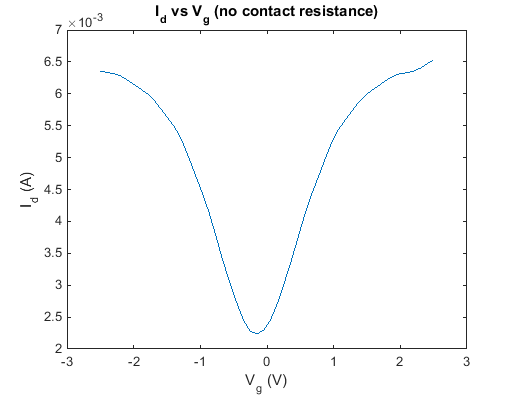
\includegraphics[width=0.4\textwidth]{Id_vg_png-small.png}
\caption{Drain current $I_d$ vs gate voltage $V_g$, without any contact resistance.}\label{fig:FET}
\end{figure}

Finally, contact resistance must be taken into account to obtain a final model for the current-voltage characteristics. Contact resistance values were taken from Wu's experimental results, and were both distinct for holes and electrons and dependent on channel length. As usual, the temperature was taken to be 300 K. Contact resistance measurements taken from Wu's experimental results indicate values of around 275 $~\Omega -\mu$m for electrons and 200 $~\Omega -\mu$m for holes for a 70 nm channel length device. The effect of contact resistance on the $I_d-V_d$ relation was calculated self-consistently, and the final current-voltage characteristics, with contact resistance taken into account, is displayed in Figure BLANK.

FIG

The effect of contact resistance is quite substantial but typical for 2-dimensional monolayers such as graphene, and constitutes a significant problem for the use of these 2-dimensional materials in field-effect transistors (to be further discussed in the final section "Efficacy of device").

\section*{iii.} The injection velocity is defined as follows:

$$v_{inj} = \frac{\sum_{k_x>0, ky}f_{k}v_{k}}{\sum_{k_x>0, ky}f_{k}} - \frac{\sum_{k_x<0, ky}f_{k}v_{k}}{\sum_{k_x<0, ky}f_{k}}$$

As before, this expression can be converted into an integral expression which includes $E_k$, when determining the Fermi function $f_{k}$, and $\nabla_k(E)$, when determining the velocity $v_{k}$.  Computing the integral as before using the rigorous bandstructure determined computationally, the injection velocity can be calculated as a function of $V_d$. The injection velocity $v_{inj}$ is shown as a function of $V_d$ in Figure BLANK.

\begin{figure}[h!]
\centering 
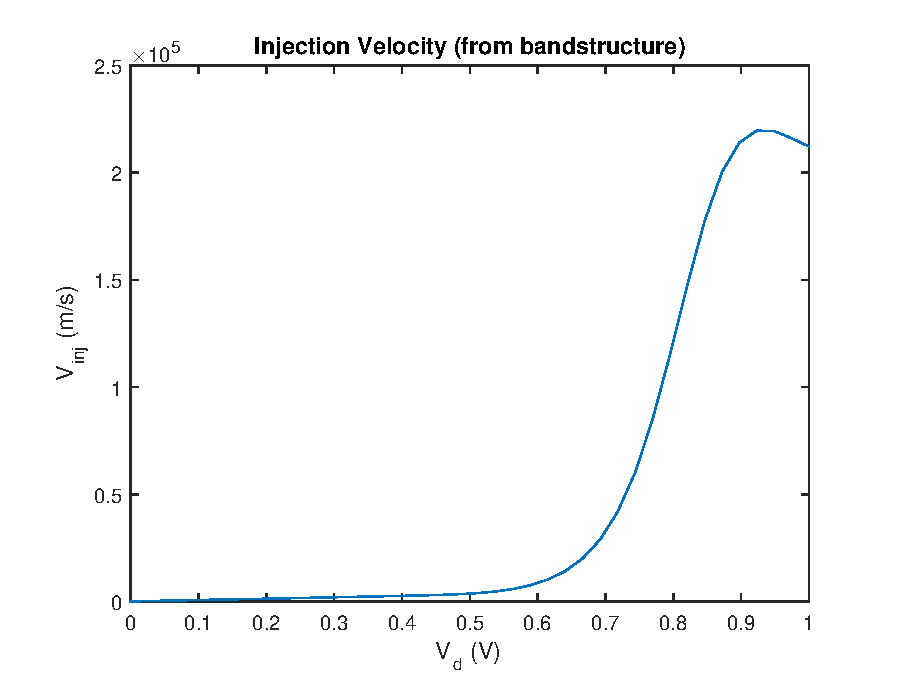
\includegraphics[width=0.4\textwidth]{vinj_saturate.eps}
\caption{$V_{inj}$ vs $V_d$, calculated from the bandstructure}\label{fig:FET}
\end{figure}

As expected for a quasi-ballistic transistor, $v_{inj}$ saturates below the thermal velocity $v_{th}$, here saturating at around $m/s$ at a drain voltage of $V_d=0.9$ V. 

It is worth noting that in traditional FETs made of semiconductors with bandgaps, $v_{inj}$ cannot exceed $v_{th}$ assuming the material is non-degenerately doped; that is, the Fermi level $E_f$ is greater than $3k_BT$ eV away from the conduction band $E_c$. Bulk graphene does not have a bandgap (as discussed in Boykin), so no such non-degenerate assumption can  be made, yet in this simulation $v_{inj}$ still saturates below $v_{th}$.

This injection velocity relationship, calculated directly from the dispersion relation, may be compared with the injection velocity calculated using an effective mass approximation. Graphene is notable because, due to the non-parabolic shape of its bandstructure around the Dirac point, one cannot obtain an effective mass\cite{ariel2012} using the conventional definition $m^{*} = \hbar^2(\frac{d^2E(k)}{dk^2})^{-1}$. 

Instead we proceed with an alternative definition $m^{*} = \hbar^2k(\frac{dE(k)}{dk})^{-1}$. This is based on the linear bandstructure of graphene in a small region around the Dirac point. Using the usual effective mass approximation that $E=\frac{\hbar^2k_x^2}{2m^{*}}$. The Fermi velocity of graphene is set to $v_f = 10^6 m/s$ as extracted from the band structure previously. From this point, we can derive the forward and backward scattering components of current as follows. 

$$I = -2ew[\sum_{kx>0,ky}{f_kv_k} - \sum_{kx<0,ky}{f_kv_k}]$$
\vspace{1em}

\begin{figure}[h!]
\centering 
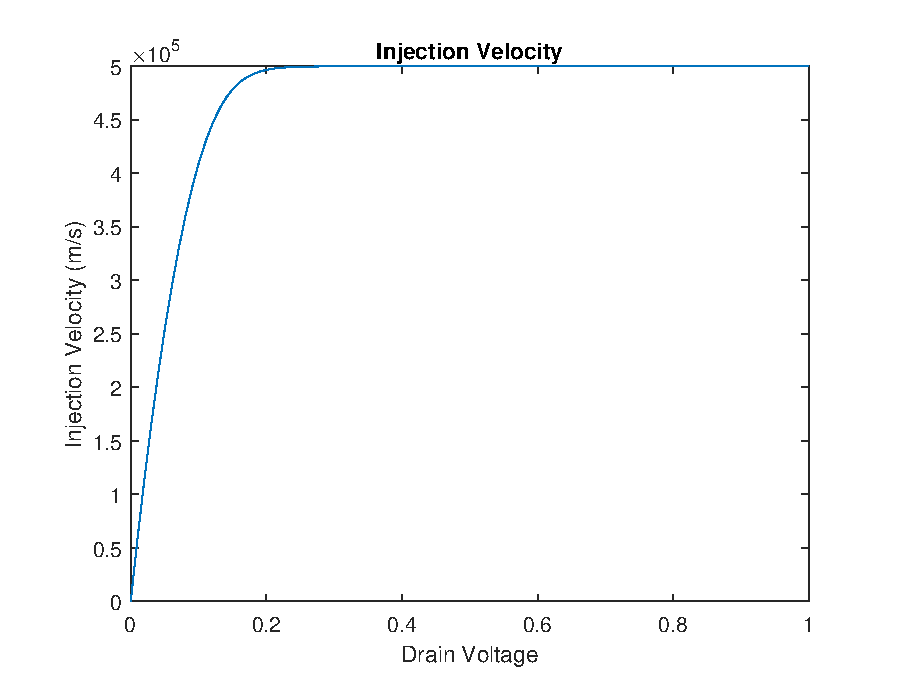
\includegraphics[width=0.4\textwidth]{Injection_Velocity.eps}
\caption{$V_{inj}$ vs $V_d$, calculated using effective mass approximation}\label{fig:FET}
\end{figure}



\section*{iv.}
Proceeding again from Wu's experimental results, the effective mobility $\mu_{eff}$ for a device with 70 nm channel length is about $1250 \frac{cm^2}{V\cdot s}$ for electrons and $800 \frac{cm^2}{V\cdot s}$ for holes.

From the mobility $\mu$ the mean free path $\lambda$ can be calculated using the formula

$$\lambda = \frac{2\mu\frac{k_BT}{q}}{v_{th}}$$

As implied from the term, analyzing device data with low-field mobility are problematic at higher electric fields in the channel caused by higher applied drain voltages.

\section*{v.}

\section*{Efficacy of device}

\begin{thebibliography}{9}

\bibitem{wu2010}
  Wu, Y.Q. et al.,
  \textit{"RF Performance of Short Channel Graphene FET"}.
  Tech. Dig Int. Electron Devices Meeting,
  pp 226-228,
  2010.
  
\bibitem{meric2011}
  Meric, I. et al.,
  \textit{"Channel Length Scaling in Graphene Field-Effect Transistors Studied with Pulsed Current-Voltage Measurements"}.
  Nano Letters 11 (3),
  1093-1097,
  (2011).
  
  \bibitem{boykin2011}
  Boykin, T. et al.,
  \textit{"Accurate six-band nearest-neighbor tight-binding model for the $\pi$ bands of bulk graphene and graphene nanoribbons."}.
  Journal of Applied Physics,
  109.10,
  (2011).
  
    \bibitem{ariel2012}
  Ariel, V. and A. Natan,
  \textit{"Electron Effective Mass in Graphene."}.
  arXiv:1206.6100,
  (2012).
  
  \bibitem{ballistic2002}
  Rahman, A. et. al.,
  \textit{"Theory of Ballistic Nanotransistors"}.
   IEEE Transactions on Electron Devices:50.9,
   1853-1864,
    (2003).
    
  \bibitem{slaterkoster1954}
  Slater, J.C., and G.F. Koster.,
  \textit{"Simplified LCAO method for the periodic potential problem."}.
   Physical Review 94.6,
    (1954): 1498.
    
  \bibitem{meric2008}
  Meric, I. et al.,
  \textit{"Current saturation in zero-bandgap, top-gated graphene field-effect transistors."}.
   Nature Nanotechnology 3 (11),
  654-659,
  (2008).
  
  \bibitem{chauhan2011}
  Chauhan, J. and J. Guo.,
  \textit{"Inelastic phonon scattering in graphene FETs."}.
   IEEE Transactions on Electron Devices 58 (11),
  3997-4003,
  (2011).
  
\end{thebibliography}


\end{document}
